\chapter{Subject and definitions}
\section{Subject presentation}
\paragraph{3D Musical instruments}
At the \ac{SCRIME} and \ac{LaBRI}, three-dimensional musical instruments have been implemented within the context of research in interactive virtual reality and music computing. 

The \brand{Drile} \cite{berthaut2010drile} is a 3D musical instrument which allows manipulation of the structure of a song using \gls{livelooping}, in an immersive virtual reality scene.

The \brand{Aerial Percussion} is a 3D musical instrument which generates sounds using the position in space of sensors which are put at the end of drumsticks. Virtual 3D shapes like cubes, cylinders, are positionned around the instrument and the musician. According to the position, the orientation, and the speed of the sensors, sounds are generated.

\paragraph{Objectives}
We were asked to implement a prototype of a 3D render and display device, for musical performance.
It is necessary to take into account the constraints inherent to a musical performance environment, as well as the constraints of the instruments.

Here are some constraints for the performance : 
\begin{itemize}
\item The musician has to be in front of the audience.
\item The musician requires visual cues inherent to the utilisation of the instrument, and the audience must see the instrument to understand the gestures and actions of the musician.
\end{itemize}

To enact this implementation, a precise explanation of the nature of the 3D musical instruments is required.

\paragraph{Plan for this section}
We will first make a short presentation of 3D musical instruments, present and will then define the concepts of immersivity and interactivity.

\newpage
\section{What is a 3D musical instrument?}
A 3D musical instrument is an instrument which is designed thanks to the progress in virtual reality and computer music.
Virtual reality provides display and control methods while computer music technologies provides sound and music synthesis. The goal is to use these tools to design an instrument which would be precise, easy to handle, and have an important artistic quality.

\paragraph{Example for the Drile}
For instance, the picture \ref{fig:drile} shows a musician with special glasses, as well as joysticks with force-feedback haptic sensors (Piivert \cite{berthaut2010piivert}). 
The user handles 3D shapes in a 3D environement to influence the music generation. A specific part of this report will be dedicated to a precise study of the \brand{Drile}.

\begin{figure}[t]
\centering
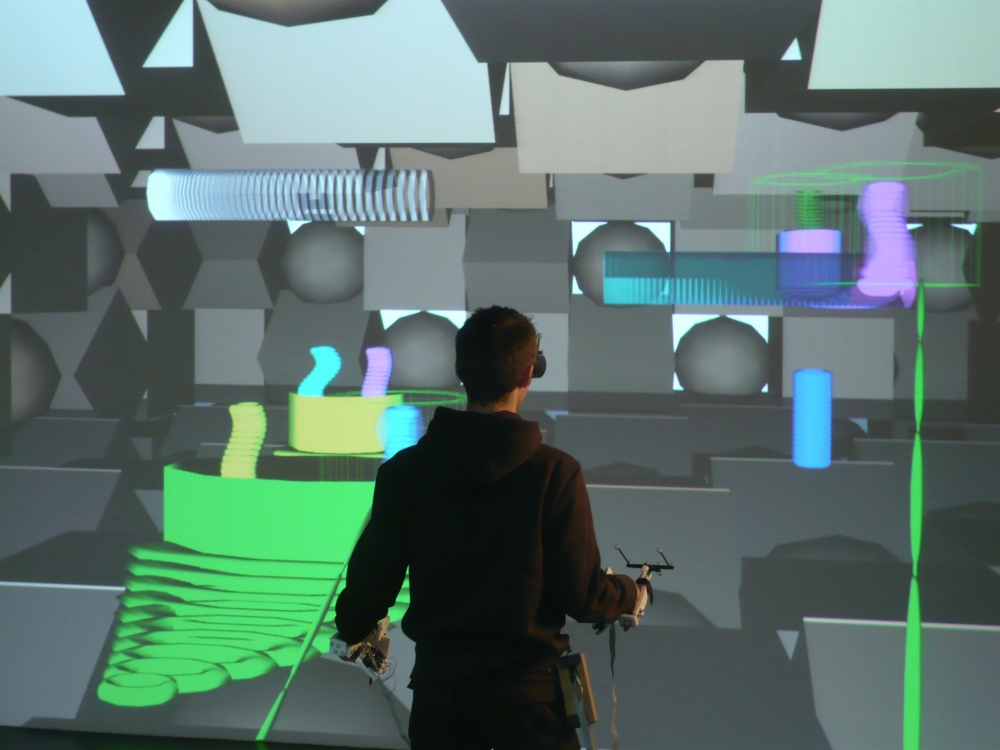
\includegraphics[scale=0.3]{image/drile.jpg}
\caption{Picture of a musician using DRILE}
\label{fig:drile}
\end{figure}

\newpage
\section{Immersion}
\paragraph{Definition}
Immersion is a psychologic state where the subject stops about taking care of its own physical state.
The immersion is quite important in virtual reality. For instance, for the Aerial Percussion, it would come down to the state the performer is when he stops thinking consciously of the disposition of the shapes he interacts with. The musician will then be immersed in the virtual 3D environment which consists in the shapes disposition.

Hence, to immerse an user, multiple parameters are accessible to the 3D instrument designer. 
They are mostly linked to the senses of the human body. In our project, we will mainly focus on vision, and more precisely on 3D display devices.

\paragraph{Interactivity \& reactivity}
Interactivity is an important aspect of the immersion capacities of a musical system.
The user is more likely to get an immersive feeling in a virtual world, if the world instantly reacts to his actions and gestures \cite{biocca1995immersive}.
This leads us to an important part of the 3D musical instrument : the interface, the controls that the performer requires to operate the instrument.

\section{Control}
In order to understand and define what is the control of a 3D musical instrument, it is necessary to think of the instrument in two different ways : 
\begin{enumerate}
\item First of all, it is a musical instrument, which implies multiples constraints :
\begin{itemize}
\item It has to be adapted to the human body shape so that the musican can manipulate it.
\item It has to be precise enough for the performer to be able to learn how to play the instrument.
\end{itemize}
\item But it is also an interactive immersive system, which means that it requires :
\begin{itemize}
\item A lot of interactivity.
\item The usage of senses for a feedback : for instance, immersive visual and haptic feedback (as well as auditive, since it is a musical instrument).
\end{itemize} 
\end{enumerate}

\paragraph{Musical instrument gestures}
In order to conceive a 3D musical instrument, it is necessary to understand the movements that the musician does while playing. For instance, the Cadoz gesture segmentation \cite{cadoz1999musique} is an attempt to differentiate different families of gestures while playing.

Cadoz defines three kinds of gestures that all come to play when playing music:

\begin{itemize}
\item Selection gestures : The musician selects a component of the instrument that he will play on. For instance, for stringed musical instruments, where the same tone can be achieved on different strings, but with a different timber, it is the choice of the string on which the note will be played.
\item Modification gestures : It is an action that modifies the physical state of the instrument. For instance, it would be the case of the guitar player who presses its hand on the guitar strings against the wood. 
\item Excitation gestures : These actions are the ones generating the actual sound of the instrument, by making the air vibe. On a guitar, it would be picking a string, and on a violin, it would be moving the bow against a string. This gesture is the one the artist can put expression inside : for instance, a violonist can press his bow softly or hardly, in order to change the nuance.
\end{itemize}

\paragraph{Control and immersion}
In order to correctly play an instrument, the user requires some kind of manipulation comfort : it must not be painful or too tiring to play. 
Hence the requirement for immersion : being immersed means that the user does not need to put effort into playing the 3D musical instrument, he becomes part of it.
An easy way to improve immersion is to make the environment react to the performer's movements. 

This can be achieved by using head tracking, with a \brand{Kinect} for instance, or a \ac{HMD}, a \ac{CAVE} or other virtual reality devices and methods like Fishtank VR \cite{robertson1997immersion}. This allows to adapt the scene's projection to the movements of the head of the user : for instance, if he turns his head to the right, the display will adapt by showing him what he would see if it was real.

Haptic feedback buttons also increase the consciousness of the user's actions, which implies an increased precision.

Florent Berthaut thought about most of these problematics while conceiving \brand{Piivert} \cite{berthaut2010piivert}, the control interface to the \brand{Drile}.
